\chapter{Attention-Based字词结合卷积循环中文短文本分类模型}
短文本分类在自然语言处理领域中扮演着重要的角色,
在垃圾信息过滤、语义分析、自动问答等任务中有着广泛的应用。
本节将通过结合基于局部感知域理论设计的卷积神经网络以及基于时间记忆理论设计的循环神经网络,
组合两种网络的优点,提出一种新型的中文短文本分类模型。该模型还引入了Attention机制等
现在最新的深度神经网络技术,并结合字向量与词向量
,优化神经网络提取出的文本特征向量,防止特征向量信息冗余或信息缺失,
增强模型在中文短文本上的分类效果。
\section{卷积循环神经特征提取网络}
根据\ref{cnn_section}小节与\ref{rnn_section}小节的介绍,我们知道
卷积神经网络和循环神经网络在特征提取方面都有优秀的表现,各有其优缺点。一方面,卷积神经网络
能够从序列数据(如文本数据)和空间数据(如图片数据)之中快速的学习本地特征,得到分类结果,
但忽略了特征的顺序,对某些数据并不适合;另一方面,循环神经网络则专门对序列数据
进行建模,但却无法并发的提取数据特征,使得模型运算较慢,无法大规模应用\citing{schmidhuber2015deep}。
针对这样的特点,本文将组合卷积神经网络与循环神经网络,把它们堆叠在一个系统中共同进行特征提取工作,
形成一个新的特征提取网络,有效的吸收两种模型的优点,同时避免其缺点。
\subsection{卷积循环神经网络整体结构}
卷积循环神经网络由卷积网络层和循环网络层两个主要模块组成,总体结构如图\ref{CLSTM}所示。
文本数据编码后,卷积网络层会对其进行处理,得到文本的初级特征图,特征图之后输入循环
网络层,进行更高一级的特征提取,并将网络中最后一个隐藏节点的输出向量作为
最终的特征向量。
\begin{figure}[h]
    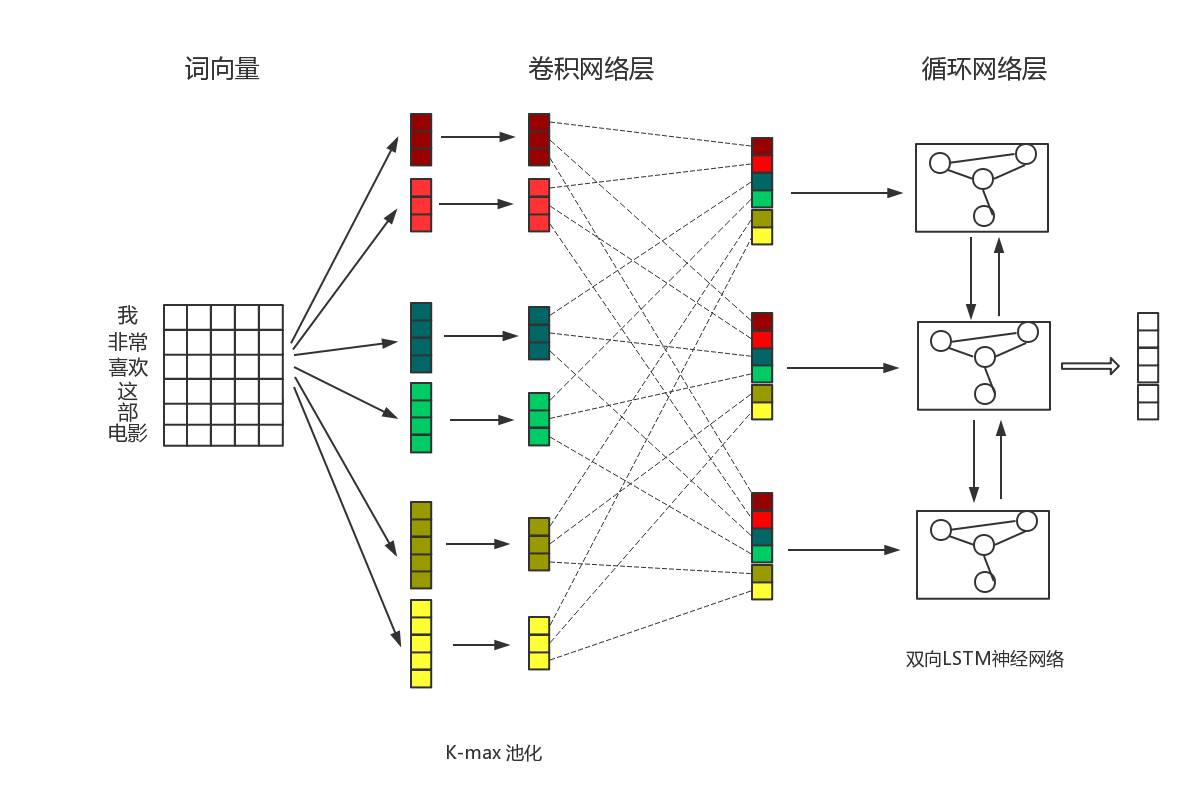
\includegraphics[scale=0.4]{picture/CLSTM.png}
    \caption{卷积循环神经网络结构图}
    \label{CLSTM}
\end{figure}
\subsection{卷积网络层}
卷积网络层的结构与普通卷积神经网络大致相同,分为卷积模块、池化模块与光栅模块。
为了适应本文研究的中文短文本数据,本文对每个模块的具体实现做出了一些调整,下面
对各个模块进行说明:

(1)卷积模块

基于文本数据的信息特征,卷积网络层的卷积模块使用窄卷积(Narrow Convolution)
作为卷积策略,避免宽卷积(Wide Convolution)的补零操作对提取文本特征造成影响。
卷积核长度分为3、4、5三种,宽度为词向量的长度,滑动步长为1,保证特征图能够包含尽可能多的文本特征。
每种卷积核生成128个,保障特征图的多样性。

(2)池化模块

由于短文本数据的长度以及卷积核的长度并不统一,卷积层产生的特征图的长度各有不同,
为了让接下来的循环网络层能够处理特征图,需要在池化模块对其进行处理,将长度统一。
本文使用k-max池化(k-max pooling)作为
池化算法,该算法是Kalchbrenner提出的动态k-max算法的前置算法\citing{kalchbrenner2014convolutional},
主要思想是对于一个给定的$k$值与特征序列$p$($p\in R^p,length(p)\geq k$),选择序列$p$中前$k$个最大值,
且保留原来序列的次序(即生成序列是原序列$p$的一个子序列)。通过k-max池化算法,卷积网络层不仅能够
接收变长的输入,同时生成的特征图也保留了相对的位置信息,提升了特征的质量。

(3)光栅模块

光栅模块主要用来整合生成的各个特征图,将其中相同位置的特征值进行合并,形成最终的特征向量,输入下面的循环网络层,
如网络结构图\ref{CLSTM}中的虚线所示。

\subsection{循环网络层}

循环神经网络依据时间对序列数据进行建模,上一个节点的数据不仅会进行输出,还会作为同一隐藏层下一个节点的输入,
隐藏层最后一个节点则能够接收到全部的文本特征数据。但是短文本分类任务需要更多的考虑文本上下文信息,单纯使用正向
循环神经网络,模型只能够依据上文信息进行分类,无法利用下文的信息,从而影响最终的分类效果。因此,本文使用
双向长短时记忆循环神经网络(Bi-directional Long Short-Term Memory,Bi-LSTM)作为循环网络层的实现,
将网络分为前向传递层与后向传递层,分别获取输入短文本的上文信息与下文信息。

Bi-LSTM网络的整体流程如图\ref{Bi-LSTM}所示,对于从上层网络传来的输入向量,网络首先将其转变为
正序序列及逆序序列两个向量,然后分别输入一个单向LSTM网络进行特征提取,得到正序特征向量与逆序特征向量,
之后将两个特征向量合并,形成最终的文本特征向量并输出到下一层网络。经过这样的处理,网络提取的特征向量既包含
上文信息又包含下文信息,能够给之后的分类网络提供更加丰富的语义信息,有效缓解了短文本数据语义信息不足的问题
,提升了分类的准确率。
\begin{figure}[h]
    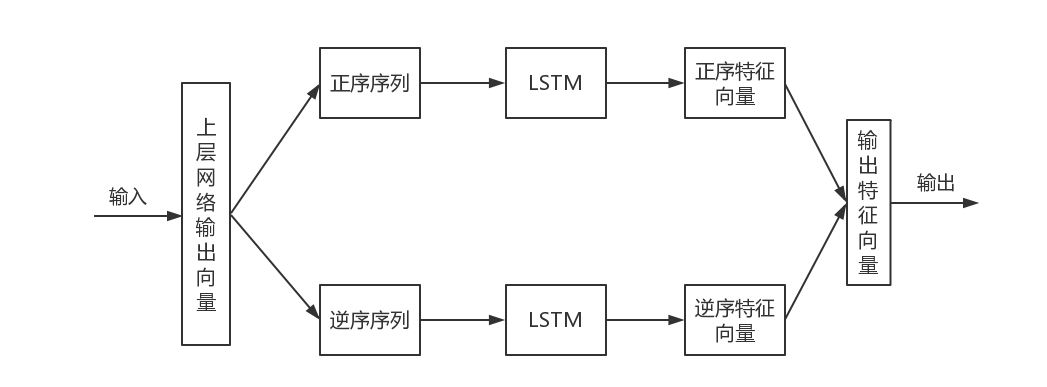
\includegraphics[scale=0.4]{picture/Bi-LSTM.png}
    \caption{Bi-LSTM网络流程图}
    \label{Bi-LSTM}
\end{figure}

\section{Attention Model}
Attention Model(注意力机制)是近几年兴起的一个新型模型,在很多场景被证明有效。
模型以认知心理学中的人脑注意力理论为核心,认为人脑在处理具体任务时,对于相关事物的注意力会集中在
某一个特定的地方,忽略其他无关的地方,而不是对每个地点分配相同的注意力。通过这样的理论,Attention Model
能够合理的分配模型的计算资源,并且还可以避免非关键数据对结果的影响。Attention Model最先在计算机视觉领域被
应用于图片识别等问题,取得了很好的成果,随后在自然语言处理领域也获得了优秀的成绩。
下面将以编码-解码模型中的Attention机制为例子,
说明Attention Model的基本知识,然后把Attention Model应用在卷积循环
神经网络当中。

编码-解码模型是自然语言处理领域中一个非常普遍的模型,它通过将输入文本编码为中间
向量,在把中间向量解码成输出向量,能够实现多种任务,如机器翻译、文本复述等。




\section{Attention-Based字词结合卷积循环中文短文本分类网络}
\section{实验结果和分析}
\section{本章小结}